\documentclass{beamer}


\usetheme{default}      % or try Darmstadt, Madrid, Warsaw, ...
\usecolortheme{default} % or try albatross, beaver, crane, ...
\usefonttheme{default}  % or try serif, structurebold, ...
\setbeamertemplate{navigation symbols}{}
\setbeamertemplate{caption}[numbered]
\setbeamertemplate{itemize items}{\raisebox{-0.em}{\scalebox{1}{\textbullet}}}


\usepackage[english]{babel}
\usepackage[utf8x]{inputenc}


%%%% adjustments to approximate RLI-template

% Colors
\definecolor{rliblue}{HTML}{002E4F}
\setbeamercolor{title}{fg=rliblue}
\setbeamercolor{frametitle}{fg=rliblue}
\setbeamercolor{normal text}{fg=rliblue}
\setbeamercolor{alerted text}{fg=rliblue}
\setbeamercolor{section in head/foot}{bg=rliblue}
\setbeamercolor{author in head/foot}{bg=rliblue}
\setbeamercolor{date in head/foot}{fg=rliblue}

% Itemize environment
\setbeamertemplate{itemize item}{\color{rliblue}$\blacktriangleright$}
\setbeamertemplate{itemize subitem}{\color{rliblue}$\blacktriangleright$}
\setbeamercolor{enumerate item}{fg=rliblue}
\setbeamercolor{enumerate subitem}{fg=rliblue}

% Fonts
\setbeamerfont{author}{size={\fontsize{10}{10}}}

\pgfdeclareimage[width=\paperwidth]{mybackground}{pics/background.pdf}
\setbeamertemplate{title page}{
        \begin{picture}(0,0)
            \put(-29,-157){%
                \pgfuseimage{mybackground}
            }

            \put(0,-110.7){%
                \begin{minipage}[b][45mm][t]{.5\textwidth}
                    \usebeamerfont{title}{\inserttitle\par\vspace{1.cm}}
                    \usebeamerfont{author}{\insertauthor\par}
                    \usebeamerfont{institute}{\insertinstitute\par}
                    \usebeamerfont{date}{\insertdate\par}
                \end{minipage}
            }
        \end{picture}
    }
    

\usepackage{tikz}
\addtobeamertemplate{headline}{}{%
\begin{tikzpicture}[remember picture,overlay]
\node at([shift={(.40\paperwidth,-.80)}]current page.north) {
\includegraphics[scale=0.1]{pics/RLI_logo.pdf}};
\end{tikzpicture}}

\usepackage{multicol}


\usepackage{amsmath}
\usepackage{tikz}

% Overlays for TIKZ pictures
\tikzset{
  invisible/.style={opacity=0},
  visible on/.style={alt={#1{}{invisible}}},
  alt/.code args={<#1>#2#3}{%
    \alt<#1>{\pgfkeysalso{#2}}{\pgfkeysalso{#3}} % \pgfkeysalso doesn't change the path
  },
}

\title[Yo]{\textbf{RLI Klausur Workshop} \\ Softwarearchitektur und best-practice Softwareentwicklung}
\author{Hendrik Huyskens \\
Pierre-Francois Duc\\
Guido Pleßmann\\}
\institute{Reiner Lemoine Institut}
\date{24. September 2019}

\begin{document}

\begin{frame}
  \titlepage
\end{frame}

\begin{frame}{Agenda des Workshops}
 \begin{enumerate}
  \item Einführung: Software design und Clean Architecture
  %\item Setup a Python project with Cookiecutter
  \item Tutorial: Test-Driven Development (TDD)
  \item Unit Tests
  \item Wrap-up
 \end{enumerate}

\end{frame}

\begin{frame}{Software design}
In Anlehnung an das Buch \emph{Clean architectures in Python} (L. Giordani, 2019)
 
 \vspace{15pt}
 \begin{itemize}
  \item Methoden um Lösungen für Probleme zu finden
  \item \emph{Patterns}\footnote{\emph{Design Patterns: Elements of Reusable Object-Oriented Software},Erich Gamma, Richard Helm, Ralph Johnson, John Vlissides, 1994}: formalisierte best-practice Vorgehensweisen
  \item Versteh warum eine Methode zu einer Lösung führt und pass' sie für dich an!
 \end{itemize}
\end{frame}

\begin{frame}{Software Architektur}

\begin{itemize}
 \item Produktionssysteme (z.B. software packages) bestehen auf Komponenten und Verbindungen
 \item In einem Prozess beschreibt die Architektur wie Komponenten miteinander verbunden sind -- immer auf einem bestimmten \emph{Zoom Level}
 \item Durch reinzoomen werden die Details Boxen, die zuvor Blackboxen mit Verbindungen ihrer Inputs und Outputs waren, sichtbar
\end{itemize}

\end{frame}


\begin{frame}{Architekturbeispiel: Shop}
% Mit TIKZ verschiedene Zoom Level auf den Prozess des Shopbetriebs grafisch darstellen



\tikzstyle{format} = [draw, thin, fill=blue!20, minimum width=2cm, minimum height=2cm]

\begin{figure}
 \begin{tikzpicture}[node distance=4cm, auto, thick]
  \node[format] (Laden) {Laden};
  \node[format, visible on=<2->] [right of=Laden] (Kunde) {Kunde};
  \draw[<-, transform canvas={yshift=15pt}, visible on=<3->] (Laden) -- (Kunde) node[midway] {Geld};
  \draw[<-, transform canvas={yshift=-15pt}, visible on=<4->] (Kunde) -- (Laden) node[midway] {Waren};
\end{tikzpicture}

\end{figure}


\end{frame}


\begin{frame}{Clean architecture}
 \begin{quote}
  
The clean architecture is the opposite of spaghetti code, where everything is interlaced and there
are no single elements that can be easily detached from the rest and replaced without the whole
system collapsing.
 \end{quote}
 
 \begin{itemize}
  \item Was befindet sich wo und warum?!
  \item Es gibt keine Wunderarchitektur die Universal angewandt werden kann
  \item Eher Prinzipien, die auf das spezielle Problem angepasst, verwendet werden können
 \end{itemize}

\end{frame}


\begin{frame}{Clean architecture}

% TODO: Was bedeuten die verschiedenen Level anhand eines Beispiels?

 \begin{figure}
 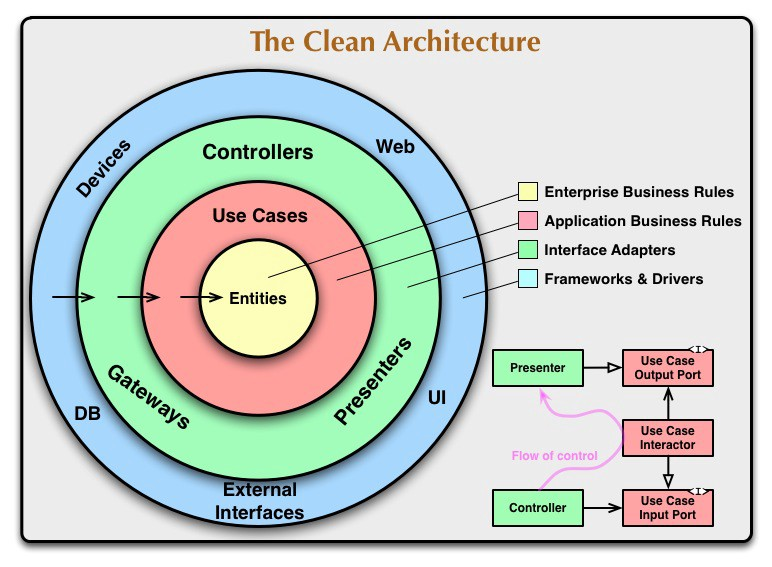
\includegraphics[width=.9\textwidth]{pics/Clean_architecture_circle.jpeg}
\caption{Source: Uncle Bob (\url{https://blog.cleancoder.com})}
\end{figure} 

\end{frame}


\begin{frame}{Clean architecture}

% Links
% https://www.freecodecamp.org/news/a-quick-introduction-to-clean-architecture-990c014448d2/
% https://www.codingblocks.net/podcast/clean-architecture-make-your-architecture-scream/
% https://blog.cleancoder.com/uncle-bob/2012/08/13/the-clean-architecture.html


\begin{columns}
 
\begin{column}{0.65\textwidth}
 \begin{figure}
 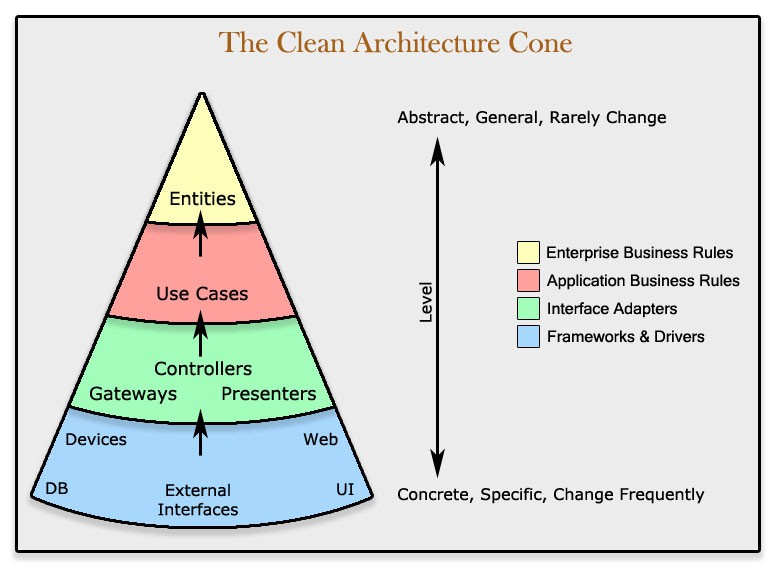
\includegraphics[width=\textwidth]{pics/Clean_architecture_cone.jpeg}
\caption{Source: Michael Outlaw (\url{https://www.codingblocks.net})}
\end{figure} 
\end{column}

\begin{column}{0.45\textwidth}
 
 \begin{itemize}
  \item Innere (abstraktere) Level kennen die äußeren Level nicht $\rightarrow$ Kommunikation über API
  \item Data flow von außen nach innen
  \item Dependencies zeigen nach innen
 \end{itemize}
\end{column}
\end{columns}
\vspace{15pt}
% Welche Klassen/Functions gehören gemeinsam in ein Level?
\end{frame}


\begin{frame}{Heutiger Workshop}
 \emph{Und wie bringen wir das heute alles unter?}
 
 \vspace{10pt}
 
 Antwort: gar nicht.\\ Wir behandeln heute Test-Driven Development (TDD) und Unit Tests. Am Ende des Workshops sprechen wir über Anschlussveranstaltungen
\end{frame}


\begin{frame}{Unit Tests: Idea}
Goal:
\begin{itemize}
\item Isolate each part of the program and show that the individual parts are correct
\item Allows refactoring of code at a later date, and makes sure the module is still working correctly
\end{itemize}
How:
\begin{itemize}
\item Many small independent and isolated tests
\item Automated tests run by developer
\item Used in TDD
\end{itemize}
\end{frame}

\begin{frame}{Unit Tests: Rules}
Unit tests should be:
\begin{description}
\item[small] e.g. concentrate on single criteria, so that failing of a test directly points to underlying error \\
Rule of thumb: Consider if the test is a logical AND between conditions or a logical OR . In the former case go for multiple assertions, in the latter create multiple test functions.
\item[fast] in order to run whole test set after each change/save to the code
\item[idempotent] e.g. should be order-independent and not rely on each other
\item[isolated] e.g. should be independent of environment or external APIs
\end{description}
\end{frame}

\begin{frame}{Test flows and types}
A component deals with several messages\footnote{Link: \url{https://speakerdeck.com/skmetz/magic-tricks-of-testing-railsconf?slide=38}}.
Messages can be differentiated into \textit{incoming}, \textit{outgoing} and \textit{private} messages and two different types (\textit{query} and \textit{command}).\\
\hfill\\
Message flows can be described by tuple \textit{(source, origin)}:
\begin{description}
\item[Incoming] (outside, self)
\item[Outgoing] (self, outside)
\item[Private] (self, self)
\end{description}
Message types:
\begin{description}
\item[Query] Return something, change nothing
\item[Command] Return nothing, change something
\end{description}
\end{frame}

\begin{frame}{Test flows and types}
How to test those 6 cases (3 flows x 2 types)?
\begin{description}
\item[Incoming query] \hfill\\
 Easy test; assert result of query
\item[Incoming command] \hfill\\
Call command and check changes by query
\item[Outgoing query/command] \hfill\\
External API not part of test, so mock external API and check only if query/command is sent
\item[Private query/command] \hfill\\
Do not test!\\
Implicitly tested by incoming/outgoing tests; test only if you think you should for some reason!
\end{description}
\end{frame}

\begin{frame}{Test flows and types: Summary}
\centering\begin{tabular}{ l c c}
  \textbf{Flow} & \textbf{Type} & \textbf{Test?} \\
  \hline
  Incoming & Query & Yes \\
  Incoming & Command & Yes \\
  Outgoing & Query & Mock \\
  Outgoing & Command & Mock \\
  Private & Query & No/Maybe \\
  Private & Command & No/Maybe \\
\end{tabular}
\end{frame}

\begin{frame}{Other Tests}
\begin{description}
\item[Integration Test] \hfill\\
Occurs after unit testing; combines multiple unit tests to a group and tests group outcome.\\
Example:\\
Login at GUI $\rightarrow$ API call $\rightarrow$ DB check $\rightarrow$ login
\item[Regression Test] \hfill \\
Re-running functional and non-functional tests to ensure that previously developed and tested software still performs after a change.
\item[Smoke Test] \hfill\\
Smoke tests are a subset of test cases that cover the most important functionality of a component or system, used to aid assessment of whether main functions of the software appear to work correctly.
\item[...]
\end{description}
\end{frame}


\begin{frame}{Wrap-up}

\centering \LARGE Warum sollte ich TDD verwenden, obwohl es viel mehr Zeit braucht???
 
\end{frame}


\begin{frame}{Follow-up: nächste Workshops}
Alle sind willkommen beizutragen!

\vspace{15pt}

Zum Beispiel Teile aus diesen beiden Büchern
 \begin{itemize}
  \item \emph{Clean architectures in Python}
  \item \emph{Design Patterns: Elements of Reusable Object-Oriented Software}
 \end{itemize}

 \vspace{15pt}
 
 Sprecht Hendrik an, er wird das koordinieren
 
\end{frame}


\begin{frame}{Feedback}
\LARGE Was war gut? Was könnte besser sein? 
\end{frame}



\end{document}

